% \section{202109-2 非零段划分}

% \subsection*{题目描述}

$A_1, A_2, \cdots, A_n$ 是一个由 $n$ 个自然数(非负整数)组成的数组。
我们称其中 $A_i, \cdots, A_j$ 是一个非零段,当且仅当以下条件同时满足:

\begin{itemize}
    \item $1 \le i \le j \le n$;
    \item 对于任意的整数 $k$,若 $i \le k \le j$,则 $A_k > 0$;
    \item $i = 1$ 或 $A_{i-1} = 0$;
    \item $j = n$ 或 $A_{j+1} = 0$。
\end{itemize}

下面展示了几个简单的例子:

\begin{itemize}
    \item $A = [3, 1, 2, 0, 0, 2, 0, 4, 5, 0, 2]$ 中的 $4$ 个非零段依次为 $[3, 1, 2]$、$[2]$、$[4, 5]$ 和 $[2]$;
    \item $A = [2, 3, 1, 4, 5]$ 仅有 $1$ 个非零段;
    \item $A = [0, 0, 0]$ 则不含非零段(即非零段个数为 $0$)。
\end{itemize}

现在我们可以对数组 $A$ 进行如下操作:
任选一个正整数 $p$,然后将 $A$ 中所有小于 $p$ 的数都变为 $0$。
试选取一个合适的 $p$,使得数组 $A$ 中的非零段个数达到最大。
若输入的 $A$ 所含非零段数已达最大值,可取 $p=1$,即不对 $A$ 做任何修改。

\subsection*{输入格式}

从标准输入读入数据。

输入的第一行包含一个正整数 $n$。

输入的第二行包含 $n$ 个用空格分隔的自然数 $A_1, A_2, \cdots, A_n$。

\subsection*{输出格式}

输出到标准输出。

仅输出一个整数,表示对数组 $A$ 进行操作后,其非零段个数能达到的最大值。

\examplebox*{\lstinputlisting[frame=none]{data/23/2-1.in}}{\lstinputlisting[frame=none]{data/23/2-1.out}}

$p = 2$ 时,$A = [3, 0, 2, 0, 0, 2, 0, 4, 5, 0, 2]$,$5$ 个非零段依次为 $[3]$、$[2]$、$[2]$、$[4, 5]$ 和 $[2]$;此时非零段个数达到最大。

\examplebox*{\lstinputlisting[frame=none]{data/23/2-2.in}}{\lstinputlisting[frame=none]{data/23/2-2.out}}

$p = 12$ 时,$A = [0, 0, 20, 0, 0, 0, 0, 15, 0, 20, 0, 0, 0, 15]$,$4$ 个非零段依次为 $[20]$、$[15]$、$[20]$ 和 $[15]$;此时非零段个数达到最大。

\examplebox*{\lstinputlisting[frame=none]{data/23/2-3.in}}{\lstinputlisting[frame=none]{data/23/2-3.out}}

$p = 1$ 时,$A = [1, 0, 0]$,此时仅有 $1$ 个非零段 $[1]$,非零段个数达到最大。

\examplebox*{\lstinputlisting[frame=none]{data/23/2-4.in}}{\lstinputlisting[frame=none]{data/23/2-4.out}}

无论 $p$ 取何值,$A$ 都不含有非零段,故非零段个数至多为 $0$。

\subsection*{子任务}

$70\%$ 的测试数据满足 $n \le 1000$;

全部的测试数据满足 $n \le 5 \times 10^{5}$,且数组 $A$ 中的每一个数均不超过 $10^{4}$。




\subsection{\texorpdfstring{$70\%$}{70\%} 数据——模拟}

\subsubsection{思路}

题目中说明 $A_i\in[0, 10000]$。当 $p>10000$ 后,$A$ 数组则成为全 $0$ 数组,
所以我们只需考虑 $k\in[1, 10000]$ 时的非零段个数,不妨设 $m=10000$。

我们可以针对每一个 $p$,计算出 $A$ 数组的情况,进而计算非零段的个数,不断更新答案。
在维护 $A$ 数组的时候,我们可以让 $p$ 递增更新。
这样在 $p$ 更新的时候,只需要将 $A_i=p-1$ 处更新为 $0$ 即可。

时间复杂度 $\mathrm{O}(nm)$。

\subsection{\texorpdfstring{$100\%$}{100\%} 数据——避免不必要更新}

\subsubsection{思路}

在上个做法中,时间主要浪费在了对 $A$ 数组的更新与重复计算非零段上。
对于每一个非零 $A_i$,随着 $p$ 逐渐增大,其最多改变一次,即变为 $0$。
而在上面的方法中,我们忽略了这个条件,每次都对所有的元素进行检查,无论其是否为 $0$。

考虑每个 $A_i$ 变为 $0$ 时对非零段个数的贡献。
为了简化后续讨论,这里给出一个推论:

\begin{corollary}[相邻相等元素与单个元素等价] \label{cor:adjacent-same-element-equals-one-element}
    对于一段值相同的区间,可以把它们看做成其中任意的一个元素。

    这一点很好理解:既然值相同,那么这一段在变为 $0$ 时必然是同时改变。
\end{corollary}

通过以上推论,我们先缩小 $A$ 数组的元素个数,直到任意相邻两个元素都不同,之后考虑每个元素对整体的贡献。
只看元素本身看不出什么,一种思路是查看与之相邻的两个元素。

\begin{figure}[H]
    \centering
    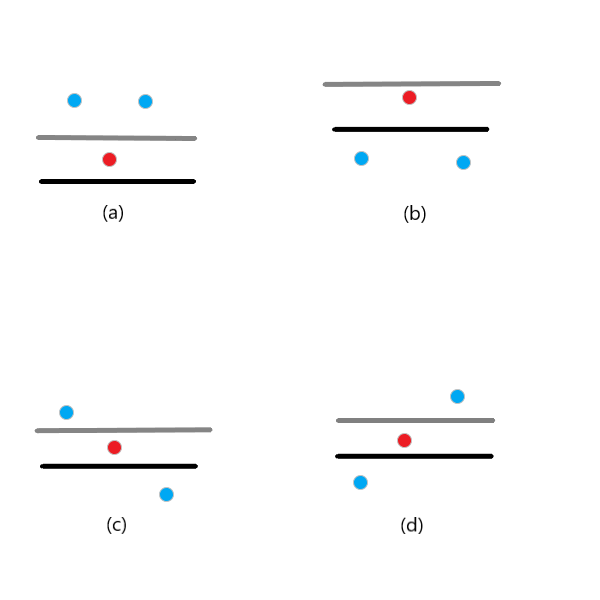
\includegraphics[width=0.6\textwidth]{image/23/2-1.png}
    \caption{相邻元素的四种情况}
\end{figure}

如图,红色点代表将要变为 $0$ 的元素,蓝色点为相邻两个元素;黑线以下为目前变为 $0$ 的元素。我们对以上四种情况进行分类讨论:

\begin{enumerate}
    \item 当左右相邻元素均大于中间元素时:当中间元素变为 $0$ 时,原本一个非零段分成了两个非零段,对非零段个数贡献 $+1$;
    \item 当左右相邻元素均小于中间元素时:当中间元素变为 $0$ 之前,左右元素均已变成 $0$,中间元素是孤立的非零段,在中间元素变为 $0$ 后,非零段个数减少,对非零段个数贡献 $-1$;
    \item 其他两种情况:相当于某个非零段的边界去掉了一个元素,对非零段个数无影响。
\end{enumerate}

针对边界元素而言,可以将其缺失的相邻元素视为 $0$。

同时,考虑到我们只需要求解非零段的个数,并不需要输出对应 $A$ 数组的状态,我们可以将每个元素的贡献(当然只有在对应 $p=A_{i}+1$ 时才会有贡献)累加,成为每个 $p$ 对应的贡献。
这样我们就可以先求出初始状态的非零段个数,之后随着 $p$ 增加利用之前求出的贡献进行更新,就可以比较快速地解决。

求出每个元素的贡献、并累加到对应 $p$ 的复杂度为 $\mathrm{O}(n)$,计算每一个 $p$ 的最后贡献的复杂度为 $\mathrm{O}(m)$,整体复杂度 $\mathrm{O}(n+m)$。

\subsubsection{C++实现}

\lstinputlisting[language=c++]{code/23/202109-2-100.cpp}